\subsection[]{Verifikation der Funktion eines phasenempfindlichen Gleichrichters}
Mit dem linken Ausgang des Funktionsgenerators (ohne die Beschriftung \enquote{phase shift}) lassen sich die Spannungsamplituden variieren.
%5.1 so semi erfüllt(?)
%
Im nächsten Schritt wird der Schaltplan \textbf{SCHALTPLAN REFERENZIEREN} aufgebaut,
um die Funktionsweise eines phasenempfindlichen Gleichrichters zu verifizieren.
Dies findet ohne Verwendung des Tiefpasses statt.
Mit dem Phasenschieber werden insgesamt fünf verschiedene Phasenverschiebungen $\phi$ eingestellt,
die in Abbildung \ref{fig:phasenunterschiede} einzusehen sind.
%
\begin{figure}%
    \begin{subfigure}{0.5\textwidth}%
    \centering%
    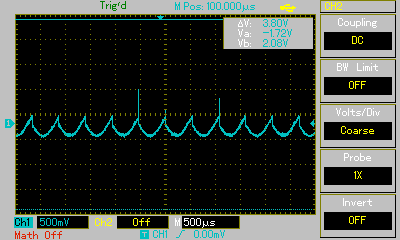
\includegraphics[width = 7.3cm]{./Oszilloskop Bilder/png/5.2/1 MAP002.png}%
    \caption{$\phi = \qty[]{0}{\degree}$}%
    \label{fig:phase1}%
    \end{subfigure}%
    %
    \hfill% Fills available space in the center -> space between figures
    \begin{subfigure}{0.5\textwidth}%
    \centering%
    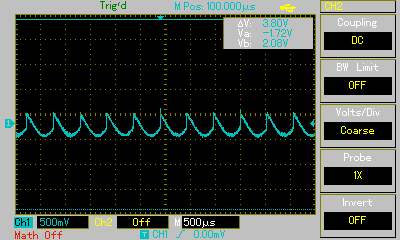
\includegraphics[width = 7.3cm]{./Oszilloskop Bilder/png/5.2/2 MAP003.png}%
    \caption{$\phi = \qty[]{45}{\degree}$}%
    \label{fig:phase2}%
    \end{subfigure}%
    %
    \hfill
    \begin{subfigure}{0.5\textwidth}%
    \centering%
    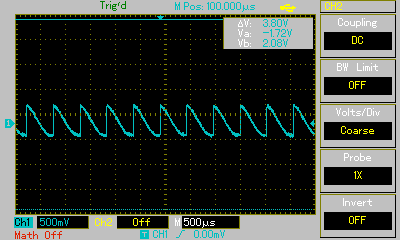
\includegraphics[width = 7.3cm]{./Oszilloskop Bilder/png/5.2/3 MAP004.png}%
    \caption{$\phi = \qty[]{90}{\degree}$}%
    \label{fig:phase3}%
    \end{subfigure}%
    %
    \hfill% Fills available space in the center -> space between figures
    \begin{subfigure}{0.5\textwidth}%
    \centering%
    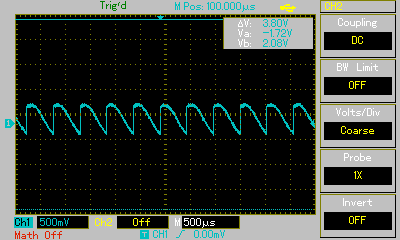
\includegraphics[width = 7.3cm]{./Oszilloskop Bilder/png/5.2/4 MAP005.png}%
    \caption{$\phi = \qty[]{135}{\degree}$}%
    \label{fig:phase4}%
    \end{subfigure}%
    %
    \hfill
    \begin{subfigure}{0.5\textwidth}%
    \centering%
    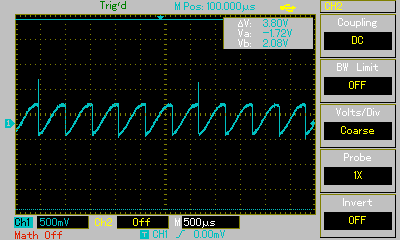
\includegraphics[width = 7.3cm]{./Oszilloskop Bilder/png/5.2/5 MAP006.png}%
    \caption{$\phi = \qty[]{180}{\degree}$}%
    \label{fig:phase5}%
    \end{subfigure}%
    %
    \caption{Spannungsverläufe für unterschiedliche Phasen}%
    \label{fig:phasenunterschiede}%
\end{figure}%
%  
%Anhand der Abbildung \ref{fig:phasenunterschiede}
%
Schaltet man den Tiefpass hinzu, ergeben sich je nach Phase $\phi$ die Spannungsamplituden $U$ in Tabelle \ref{tab:u_out_tp_ohne_noise}.


%
%\begin{table}
%    \centering
%    \caption[]{Amplitude der Ausgangsspannung nach Integration}
%    \label{tab:u_out_tp_ohne_noise}
%    \sisetup{table-format=3.0}
%    \begin{tabular}[]{S S[table-format=4.1] S[table-format=4.1]}
%        \toprule
%        {$\phi / \unit[]{\degree}$} & {$U_\text{out,Ch1} / \unit[]{\milli\volt}$} & {$U_\text{average,Ch2} / \unit[]{\milli\volt}$} \\
%        \midrule
%           0 &  871.2 & -100.0 \\
%          45 &  712.8 & -100.0 \\
%          90 &  653.4 &   40.0 \\
%         135 &  613.8 &  180.0 \\
%         180 &  455.4 &  280.0 \\
%         225 &  950.4 &  260.0 \\
%         270 & 1190   &  140.0 \\
%         300 &  990.0 &   60.0 \\
%         315 & 1170   &    0.0 \\
%         330 & 1030   &  -60.0 \\
%        \bottomrule
%    \end{tabular}
%\end{table}

\begin{table}
    \centering
    \caption[]{Amplitude der Ausgangsspannung nach Integration}
    \label{tab:u_out_tp_ohne_noise}
    \sisetup{table-format=3.0}
    \begin{tabular}[]{S c S[table-format=2.2]}
        \toprule
        {$\phi / \unit[]{\degree}$} & {$\phi / \unit[]{\radian}$} & {$U / \unit[]{\volt}$} \\
        \midrule
           0 &     0          & -0.1  \\
          45 & $    \pi / 4 $ & -0.1  \\
          90 & $    \pi / 2 $ &  0.04 \\
         135 & $ 3  \pi / 4 $ &  0.18 \\
         180 & $    \pi     $ &  0.28 \\
         225 & $ 5  \pi / 4 $ &  0.26 \\
         270 & $ 3  \pi / 2 $ &  0.14 \\
         300 & $ 5  \pi / 3 $ &  0.06 \\
         315 & $ 7  \pi / 4 $ &  0    \\
         330 & $ 11 \pi / 6 $ & -0.06 \\
        \bottomrule
    \end{tabular}
\end{table}

%-100.0
%-100.0
%  40.0
% 180.0
% 280.0
% 260.0
% 140.0
%  60.0
%   0.0
% -60.0

%fit mit cos(...) machen